\section{Partial Derivatives}
\noindent
The single-variable calculus idea of tangent lines doesn't work for higher dimensional surfaces because we can draw many different lines that are tangent to the surface, depending on which plane we use to slice the surface. That is, from which direction we approach the surface.
\subsection{Partial Derivatives of X, Y, and Z}
\noindent
It's common to look at the derivative when slicing a surface in the yz, xz, and xy planes. These are called partial derivatives.\\

\noindent
To compute $\frac{\partial}{\partial x}{f(x,y)}$, we take the derivative with respect to $x$ as if $y$ is constant. Formally,
\begin{equation*}
	\frac{\partial}{\partial x}f(x,y) = \lim_{h \to 0}{\frac{f(x+h,y)-f(x,y)}{h}}
\end{equation*} 
and 
\begin{equation*}
	\frac{\partial}{\partial y}f(x,y) = \lim_{h \to 0}{\frac{f(x,y+h)-f(x,y)}{h}}
\end{equation*}

\noindent
We also use the shorthand $\frac{\partial}{\partial x}=f_x$ and $\frac{\partial}{\partial y}=f_y$. This shorthand can be extended to higher-order derivatives so that $\frac{\partial}{\partial y}\left(\frac{\partial}{\partial x}f(x,y)\right)=f_{xy}$.

\noindent
Fubini's Theorem (also called Tonelli's or Clairaut's Theorem) says $f_{xy} = f_{yx}$, $f_{xz} = f_{zx}$, and $f_{yz} = f_{zy}$. It extends into higher-order mixed partial derivatives, saying that two mixed partial derivatives of a function are equal as long as they both differentiate the same number of variables the same number of times. So, $f_{abcdab} = f_{aacdbb}$.
\subsection{Tangent Planes}
\noindent
Although the tangent lines at a point on a surface can all be different depending on from which direction one approaches a point, all of these tangent lines lie in the same plane, defining the tangent plane.
This means that the tangent plane to $z = f(x, y)$ at $(x_0,y_0)$ has the following properties:
\begin{itemize}
	\item The z-value of the tangent plane at $(x_0, y_0)$ is the same as $f(x_0, y_0)$.
	\item The value of the first-order partial derivatives of the tangent plane at $(x_0, y_0)$ should match those of $f(x_0, y_0)$.
\end{itemize}

\noindent
The general form of a plane at $(x_0, y_0, z_0)$ is
\begin{equation*}
	P(x,y) = A(x-x_0) + B(y-y_0) + z_0.
\end{equation*}
We want $P_x = f_x$ and $P_y = f_y$.
This means that $P_x = f_x = A$ and $P_y = f_y = B$.
Rewriting,
\begin{equation*}
	P(x,y) = f_x(x-x0) + f_y(y-y_0) + z_0.
\end{equation*} 
The normal vector is $\langle \pm f_x,\pm f_y, \mp 1\rangle$.
So, the point normal form of the plane is 
\begin{equation*}
	\langle -f_x, -f_y, 1\rangle \cdot \langle x-x_0, y-y_0, z-f(x_0,y_0) \rangle = 0.
\end{equation*}

\begin{figure}[H]
	\centering
	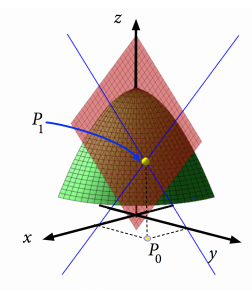
\includegraphics[width=0.5\textwidth]{./Images/differentialMultivariableCalculus/tangent_plane.png}
	\caption{Tangent plane}
\end{figure}

\subsection{Linear Approximations}
\noindent
Since $\partial z = f_x\partial x + f_y\partial y$, we can approximate $\Delta z$ (the change in any function) as $\Delta z \approx f_x\Delta x + f_y\Delta y$, since values of $f$ and the tangent plane are close. We an rewrite this approximation as a dot product: $\Delta z \approx \langle f_x, f_y\rangle \cdot \langle \Delta x, \Delta y \rangle$.\\

For example, say a cylindrical can has a radius $r=1$ and a height $h=5$. If the radius is increased by .1 and the height is increased by 1, what is the approximate $\Delta V$?
\begin{equation*}
	V(r,h) = \pi r^2 h, V_r = 2\pi rh \text{, and } V_h = \pi r^2
\end{equation*}
\begin{equation*}
	V_{r}(1,5) = 10\pi  \text{ and } V_{h}(1,5) = \pi
\end{equation*}
\begin{equation*}
	\Delta V \approx 10\pi(.1) + \pi(1) = 2\pi	
\end{equation*}
Comparing this to the actual answer of $2.26\pi$, we see our approximation is decent.